% \usepackage[UTF8]{ctex}
% 使用%可以书写注释,在本行内%及以后的内容不会显示在编译后的PDF文件中。

\documentclass[UTF8]{ctexart}

\usepackage{CJKutf8}
\usepackage{geometry}
\usepackage{amsmath}
\usepackage{amssymb}
\usepackage{booktabs}

\usepackage{graphicx}
\usepackage{float}

\usepackage{listings}
\usepackage{color}
\usepackage{xcolor}

\definecolor{ChatGPT}{RGB}{50, 170, 168}
\definecolor{modify}{RGB}{50, 127, 168}

\newcommand{\ch}[1]{\textcolor{ChatGPT}{#1}}
\newcommand{\m}[1]{\textcolor{modify}{#1}}

\definecolor{dkgreen}{rgb}{0,0.6,0}
\definecolor{gray}{rgb}{0.5,0.5,0.5}
\definecolor{mauve}{rgb}{0.58,0,0.82}
\lstset{frame=tb,
        language=Java,
        aboveskip=3mm,
        belowskip=3mm,
        showstringspaces=false,
        columns=flexible,
        basicstyle=\ttfamily\small,
        numbers=none,
        numberstyle=\tiny\color{gray},
        keywordstyle=\color{blue},
        commentstyle=\color{dkgreen},
        stringstyle=\color{mauve},
        breaklines=true,
        breakatwhitespace=true,
        tabsize=3
}
\lstset{frame=tb,
        language=Go,
        aboveskip=3mm,
        belowskip=3mm,
        showstringspaces=false,
        columns=flexible,
        basicstyle = \ttfamily\small,
        numbers=none,
        numberstyle=\tiny\color{gray},
        keywordstyle=\color{blue},
        commentstyle=\color{dkgreen},
        stringstyle=\color{mauve},
        breaklines=true,
        breakatwhitespace=true,
        tabsize=3
}

\usepackage{tikz}
\usetikzlibrary{positioning,shapes,arrows}

\tikzset{
    class/.style={
        rectangle,
        draw=black,
        text centered,
        minimum height=3em
    },
    arrow/.style={
        ->,
        >=stealth,
        thick
    }
}

\usetikzlibrary{shapes.geometric, arrows}

\tikzstyle{startstop} = [rectangle, rounded corners, minimum width=3cm, minimum height=0.8cm,text centered, draw=black, fill=red!30]
\tikzstyle{io} = [trapezium, trapezium left angle=70, trapezium right angle=110, minimum width=3cm, minimum height=0.8cm, text centered, draw=black, fill=blue!30]
\tikzstyle{process} = [rectangle, minimum width=3cm, minimum height=0.8cm, text centered, draw=black, fill=orange!30]
\tikzstyle{decision} = [diamond, minimum width=2cm, minimum height=0.5cm, text centered, draw=black, fill=green!30]
\tikzstyle{arrow} = [thick,->,>=stealth]

% \begin{CJK}{UTF8}{gbsn}
\geometry{a4paper,scale=0.7}
\pagestyle{plain}

    \title{软件设计文档}
    \author{项目名称:升学指导}
    \date{\today}
\begin{document}

    \maketitle

    \begin{center}
        \begin{tabular}{|c|c|}
            \hline
            姓名 & 于海龙 \\	
            \hline
            学号 & 2120220695 \\	
            \hline
            完成作业共花费&72小时\\
            \hline
            ChatGPT 完成任务比例&40\%\\
            \hline
            实现软件功能预计还需要&20天\\
            \hline
        \end{tabular}

        \par
        % 注:文章中加粗标注的内容使用ChatGPT生成。
    \end{center}

    
    % \begin{abstract}
    % \end{abstract}

    \newpage
    \tableofcontents
    \newpage
    
    \section{背景介绍}
    \subsection{升学问题现状}
    \par
    \m{当学生决定进入研究生阶段时需要仔细考虑自己的职业目标、兴趣爱好和能力,以及选择最适合自己的学校、专业和导师}。这项任务存在一些困难,因为存在太多的选择,并且需要考虑非常多不同的因素,例如学校的声誉、专业的难度、导师的研究领域等等。
    
    \par
    当前的学生面临许多的升学问题,这些问题包括了学校选择、专业选择、导师选择等几个方面。作为学生,首先需要确定自己的研究方向,\m{研究方向决定了学生未来的职业发展方向和就业前景};\m{同时学生也会因为选择合适的研究方向更好地发挥自己的优势和兴趣,提高研究效率和成果质量}。学校选择也是一项重要任务,因为\m{学校的排名和声誉可以影响到研究生的就业前景和职业发展};与此同时\m{学校所在地的交通、生活条件等也需要考虑,这些因素可能会影响到研究生的生活质量和学习效果}。

    \subsection{软件开发目标}
    \par
    \m{设计一款升学指导软件的目的是帮助学生更好地规划自己的未来,解决他们在升学过程中所面临的各种问题和挑战}。目前市面上有很多升学指导的软件,\m{如考研帮、留学Go、升学宝和升学通等}。这些市面上的软件具有不同的特色,具体如下:
    
    \begin{enumerate}
        \item 考研帮:\ch{考研帮是一款专门为考研学生提供的软件,它提供了各种考研资讯、历年真题、模拟考试等服务。用户可以通过该软件获取最新的考研政策、报考指南、院校信息等,还可以参加各种在线课程和学习小组,与其他考生交流经验和心得。此外,考研帮还提供了一些实用的工具,如错题本、复习计划、考试倒计时等,帮助学生更好地备考。}
        \item 留学Go:\ch{留学Go是一款为留学生提供服务的软件,它提供了各国留学信息、申请流程、签证办理等方面的指导和建议。用户可以通过该软件了解各国的大学排名、专业设置、学费情况等信息,还可以查看各个大学的官方网站和招生简章,了解具体的申请要求和流程。此外,留学Go还提供了一些实用的功能,如语言测试、文书模板、面试技巧等,帮助学生更好地准备留学申请。}
        \item 升学宝:\ch{升学宝是一款综合性的升学指导软件,它提供了多种服务,包括选校咨询、专业选择、申请指导等。用户可以通过该软件了解各个大学的招生政策、录取标准、课程设置等信息,还可以查看各个专业的就业前景和发展趋势。此外,升学宝还提供了一些实用的功能,如职业测评、志愿填报、面试模拟等,帮助学生更好地规划自己的升学路线。}
        \item 升学通:\ch{升学通是一款为高中生和大学生提供升学指导的软件,它提供了多种服务,包括选科咨询、专业选择、大学排名等。用户可以通过该软件了解各个大学的招生政策、录取标准、课程设置等信息,还可以查看各个专业的就业前景和发展趋势。}
    \end{enumerate}

    \begin{figure}[htp]
        \centering
        \begin{tikzpicture}[node distance=1.8cm]
            \node (student) [class] {学生信息};
            \node (school) [class, below of=student] {学校信息};
            \node (major) [class, below of=school] {专业信息};
            \node (supervisor) [class, below of=major] {导师信息};
            \node (recommendation) [class, right of=school, xshift=3cm] {升学建议};
            \draw [arrow] (student) -- (recommendation);
            \draw [arrow] (school) -- (recommendation);
            \draw [arrow] (major) -- (recommendation);
            \draw [arrow] (supervisor) -- (recommendation);
        \end{tikzpicture}
        \caption{\m{获取升学推荐信息}}
        \label{fig:element}
    \end{figure}

    \par
    这几款软件存在信息来源不够全面、界面设计不简洁直观和功能不全面等问题。因此我们需要为研究生设计一款简单明了的升学指导软件,如图\ref{fig:element}所示。这款软件期待的目标包括:简洁明了的界面设计、完备的数据库设计、高效的匹配算法设计和数据安全设计。\m{一款升学指导软件可以帮助学生更好地选择适合自己的研究生阶段的学校、专业和导师,这对于他们的职业发展和人生规划非常重要,因此这款软件具有很高的实用性和价值}。

    \section{项目概述}

    \subsection{系统功能}
    \par
    该软件的主要功能是为用户提供升学建议,并提供学校、专业和导师的信息查询服务。除此之外,还需要提供用户基本信息管理、学校专业信息管理、后台管理和统计分析的功能。为了可以支持后续的学生培养计划,还可以在未来允许职场性格测试、职业发展分析等功能的接入。

    \subsection{业务描述}

    \subsubsection{用户升学建议查询}

    \par
    用户升学建议查询的主要流程包括:
    \begin{enumerate}
        \item 输入学生信息;包括学习成绩、兴趣爱好、就职意向等,为系统分析数据提供基础支持。
        \item 系统分析数据;根据学生输入的信息和数据库中的学校、专业和导师信息,执行匹配算法和推荐算法,对数据进行分析。
        \item 生成推荐列表;根据上一步分析的结果,使用Top-K策略选择推荐列表,供用户筛选。
        \item 完成选择;用户根据推荐列表完成升学选择。
    \end{enumerate}

    \begin{figure}[htp]
        \centering
        \begin{tikzpicture}[node distance=1.8cm]
          \node (start) [startstop] {开始};
          \node (input) [io, below of=start] {输入学生信息};
          \node (process1) [process, below of=input] {对数据进行分析};
          \node (decision1) [decision, below of=process1, yshift=-0.5cm] {查询相关信息};
          \node (process2a) [process, below of=decision1, yshift=-1cm] {提供学校、专业和导师的信息};
          \node (process2b) [process, below of=process2a, yshift=-0.5cm] {完成选择};
          \node (stop) [startstop, below of=process2b] {结束};
          \draw [arrow] (start) -- (input);
          \draw [arrow] (input) -- (process1);
          \draw [arrow] (process1) -- (decision1);
          \draw [arrow] (decision1) -- node[anchor=east] {yes} (process2a);
          \draw [arrow] (process2a) -- (process2b);
          \draw [arrow] (process2b) -- (stop);
          \draw [arrow] (decision1.west) -- ++(-2,0) |- node[anchor=south] {no} (input.west);
        \end{tikzpicture}
        \caption{\m{输入学生信息查询学校、专业和导师信息流程图}}
        \label{fig:flowchart0}
    \end{figure}
    
    \par
    当用户执行一次升学建议查询时,具体的流程如图\ref{fig:flowchart0}所示。

    \subsubsection{管理员更新学校专业信息}

    \par
    软件管理员更新学校专业和导师信息的主要流程包括:

    \begin{enumerate}
        \item 管理员输入学校信息;用于数据库查询学校信息并执行更新操作。
        \item 管理员输入专业信息;用于数据库查询专业信息并执行更新操作。
        \item 管理员输入导师信息;用于数据库查询导师信息并执行更新操作。
    \end{enumerate}

    \par
    当管理员用户执行一次学校、专业和导师信息更新时,具体的流程如图\ref{fig:flowchart1}所示。

    \begin{figure}[htp]
        \centering
        \begin{tikzpicture}[node distance=1.8cm]
          \node (start) [startstop] {开始};
          \node (input1) [io, below of=start] {输入学校信息};
          \node (process1) [process, below of=input1] {查找学校信息并更新};
          \node (decision1) [decision, below of=process1, yshift=-0.5cm] {专业信息更新?};
          \node (input2) [io, below of=decision1, yshift=-1cm] {输入专业信息};
          \node (process2) [process, below of=input2] {查找专业信息并更新};
          \node (decision2) [decision, below of=process2, yshift=-0.5cm] {导师信息更新?};
          \node (input3) [io, below of=decision2, yshift=-1cm] {输入导师信息};
          \node (process3) [process, below of=input3] {查找并更新导师信息};
          \node (stop) [startstop, below of=process3] {结束};
          \draw [arrow] (start) -- (input1);
          \draw [arrow] (input1) -- (process1);
          \draw [arrow] (process1) -- (decision1);
          \draw [arrow] (decision1.west) -- ++(-2,0) |- node[anchor=south] {no} (input1.west);
          \draw [arrow] (decision1.south) -- node[anchor=west] {yes} (input2.north);
          \draw [arrow] (input2) -- (process2);
          \draw [arrow] (process2) -- (decision2);
          \draw [arrow] (decision2.west) -- ++(-2,0) |- node[anchor=south] {no} (input2.west);
          \draw [arrow] (decision2.south) -- node[anchor=west] {yes} (input3.north);
          \draw [arrow] (input3) -- (process3);
          \draw [arrow] (process3) -- (stop);
        \end{tikzpicture}
        \caption{\m{更新学校和专业信息流程图}}
        \label{fig:flowchart1}
    \end{figure}

    \subsubsection{用户管理}

    \par
    用户注册、登录和登出的主要流程包括:
    \begin{enumerate}
        \item 用户注册;\m{用户需要在注册页面输入用户名、密码、电子邮件地址等信息,并提交注册请求。系统将验证用户输入的信息,如果验证通过,则创建用户账户,并将用户信息保存在用户数据库中。如果验证未通过,则系统将提示用户重新输入信息。}
        \item 用户登录;\m{用户需要在登录页面输入用户名和密码,并提交登录请求。系统将验证用户输入的信息,如果验证通过,则用户登录系统,可以访问系统提供的服务。如果验证未通过,则系统将提示用户重新输入信息。}
        \item 用户注销;\m{用户在登录状态下可以选择注销登录,退出系统。用户注销后,系统将清除用户登录信息,确保用户的账户安全。}    
    \end{enumerate}

    \par
    当用户执行一次账户注册和登录时,具体的流程如图\ref{fig:flowchart2}所示。

    \begin{figure}[htp]
        \centering
        \begin{tikzpicture}[node distance=1.8cm]
          \node (start) [startstop] {开始};
          \node (input1) [io, below of=start] {输入注册信息};
          \node (process1) [process, below of=input1] {创建用户账户};
          \node (input2) [io, below of=process1] {输入账户信息};
          \node (decision1) [decision, below of=input2, yshift=-0.5cm] {用户凭据正确?};
          \node (process2) [process, below of=decision1, yshift=-1cm] {登入};
          \node (decision2) [decision, below of=process2, yshift=-0.5cm] {保持登录?};
          \node (process3) [process, below of=decision2, yshift=-1cm] {登出};
          \node (stop) [startstop, below of=process3] {结束};
          \draw [arrow] (start) -- (input1);
          \draw [arrow] (input1) -- (process1);
          \draw [arrow] (process1) -- (input2);
          \draw [arrow] (input2) -- (decision1);
          \draw [arrow] (decision1.west) -- ++(-2,0) |- node[anchor=south] {no} (input2.west);
          \draw [arrow] (decision1.south) -- node[anchor=west] {yes} (process2);
          \draw [arrow] (process2) -- (decision2);
          \draw [arrow] (decision2.west) -- ++(-2,0) |- node[anchor=south] {no} (input2.west);
          \draw [arrow] (decision2.south) -- node[anchor=west] {yes} (process3);
          \draw [arrow] (process3) -- (stop);
        \end{tikzpicture}
        \caption{\m{用户注册与登录流程图}}
        \label{fig:flowchart2}
    \end{figure}

    \subsubsection{统计分析}
    \par
    管理员执行数据统计分析的主要流程包括:
    \begin{enumerate}
        \item 输入登录信息;\m{管理员需要在登录页面输入用户名和密码,并提交登录请求}。
        \item 验证用户身份;\m{系统将验证管理员输入的信息,如果验证通过,则管理员登录系统,可以访问统计后台数据。如果验证未通过,则系统将提示管理员重新输入信息}。
        \item 访问统计后台数据;\m{管理员登录后,可以访问统计后台数据,并从数据库中检索相关的统计数据。系统将通过管理员账户和数据库来实现这个过程,以保护管理员的隐私和安全,确保管理员可以方便地查看统计数据}。
        \item 生成并输出报告;\m{系统将检索相关的统计数据,并生成报告。报告可以显示统计数据的图表、表格和其他相关信息。生成的报告将输出给管理员。管理员可以查看报告,并根据报告中的统计数据做出正确的决策}。
    \end{enumerate}

    \begin{figure}[htp]
        \centering
        \begin{tikzpicture}[node distance=1.8cm]
          \node (start) [startstop] {开始};
          \node (input1) [io, below of=start] {管理员登录};
          \node (process1) [process, below of=input1] {认证管理员用户信息};
          \node (process2) [process, below of=process1] {链接后端数据库};
          \node (process3) [process, below of=process2] {筛选并聚合数据};
          \node (process4) [process, below of=process3] {生成数据报告};
          \node (output1) [io, below of=process4] {返回报告结果};
          \node (stop) [startstop, below of=output1] {结束};
          \draw [arrow] (start) -- (input1);
          \draw [arrow] (input1) -- (process1);
          \draw [arrow] (process1) -- (process2);
          \draw [arrow] (process2) -- (process3);
          \draw [arrow] (process3) -- (process4);
          \draw [arrow] (process4) -- (output1);
          \draw [arrow] (output1) -- (stop);
        \end{tikzpicture}
        \caption{\m{管理员查看统计数据}}
        \label{fig:flowchart3}
    \end{figure}
    当管理员用户执行一次统计数据查看操作时,主要流程如图\ref{fig:flowchart3}所示。

    \subsection{数据流程描述}
    \subsubsection{数据}
    \par
    在这个软件系统中需要记录保存和管理的数据主要包括:
    \begin{enumerate}
        \item 学生用户信息;学生用户需要提交学生升学相关的数据,包括学生的考试成绩、兴趣爱好、工作目标等内容。除此之外,还需要在数据库中存储用户的凭证信息以供登录使用。
        \item 管理员信息;系统数据库需要存储管理员的凭证信息以供登录使用,并且需要存储管理员的操作记录日志,可以在数据出现问题是及时查找问题并恢复。
        \item 学校信息;系统数据库需要保存学校信息,以供升学建议的生成。
        \item 专业信息;系统数据库需要保存专业信息,专业信息与学校信息关联,以供升学建议的生成。
        \item 导师信息;系统数据库需要保存导师信息,导师信息与学校和专业信息关联,以供升学建议的生成。
    \end{enumerate}
    \subsubsection{数据间的关系}
    \begin{figure}[h!]
        \centering
        \begin{tikzpicture}[node distance=2cm]
          \node (user) [rectangle, draw=black] {用户};
          \node (school) [rectangle, draw=black, below right=2cm and 3cm of user] {学校};
          \node (major) [rectangle, draw=black, below right=2cm and 0.5cm of user] {专业};
          \node (advisor) [rectangle, draw=black, below right=2cm and 0.5cm of school] {导师};
          \node (admin) [rectangle, draw=black, below left=2cm and 0.5cm of school] {管理员};
          \draw [->,>=stealth] (user) -- (major);
          \draw [->,>=stealth] (user) -- (school);
          \draw [->,>=stealth] (user) -- (advisor);
          \draw [->,>=stealth] (school) -- (major);
          \draw [->,>=stealth] (school) -- (advisor);
          \draw [->,>=stealth] (major) -- (advisor);
          \draw [->,>=stealth] (admin) -- (school);
          \draw [->,>=stealth] (admin) -- (advisor);
          \draw [->,>=stealth] (admin) -- (major);
        \end{tikzpicture}
        \caption{存储数据间存在的关系}
        \label{fig:relationship}
    \end{figure}

    \subsection{用户特点}
    \subsubsection{学生用户}
    \subsubsection{系统管理员}
    \subsection{运行环境要求}
    \subsubsection{前端用户界面}
    \subsubsection{后端程序}
    \subsubsection{数据库}    

    \section{基本设计概述}
    \subsection{数据存储与共享}
    \par
    对于医疗信息这种涉及个人隐私的数据来说,
    使用类似于比特币区块链网络一样的直接存储方式
    明显是不现实的,因此,区块链网络只能作为
    一个数据分布式存储的平台提供医疗数据共享服务,
    并且确保这些数据难以被某些节点恶意篡改。
    因此,这样的一个系统需要通过一些合理的加密
    手段以确保存储的数据难以被外界人员恶意读取。
    \par
    为了提供可靠的、防篡改的医疗数据存储,可以
    使用对数据进行非对称加密存储的联盟链区块链
    网络对医疗数据和个人健康数据等进行存储,通过
    管理推送软件对数据进行加密解密、
    读写和传输,并对数据的读写行为进行监管、记录,
    以便于为普通用户和医务人员
    提供即时可靠的医疗数据访问服务。同时,为
    保障用户个人信息不被恶意泄露,在非特殊情况下,
    (特殊情况指患者需要紧急救治,并且无相关人员
    能够及时全面提供患者的有效信息),
    用户的医疗信息需要在用户或其法定监护人授意的
    情况下才能被医院获取。
    \subsection{数据安全与制约机制}
    \par
    在一般情况下,医院读取用户的医疗数据需要用户或其法定监护人
    同意并授权才能访问,管理软件会对用户的个人
    身份信息进行一定程度的脱敏处理,在完成整个
    就诊流程后,数据访问将会被禁用,用户也可以
    在就诊流程中结束医院的数据访问,因此在这样
    的流程中,数据的安全可以得到一定程度上的保障。
    
    \par
    考虑到特殊情况的存在,(如患者等待接受急救等),
    用户无法及时为医院读取数据提供授权,医院又
    急需用户的医疗数据,可以允许医院临时调用用户的
    重要医疗信息和近期病历记录。如果无限制地允许
    医院临时调用用户的医疗信息,这无异于明文的
    比特币区块链网络。因此对于医院临时对读取数据
    而言,可以设计一种制约机制,
    使得医院临时读取数据的行为受到合理的约束。
    对于医院的监管,需要一个可信任的组织通过软件
    管理平台根据不同医院的实际情况,如医院的
    类型、规模、就诊人次等信息进行分析
    判断,并为不同的医院设置不同的单位时间临时
    读取上限。软件管理平台可以根据医院的历史操作
    行为为管理者提供相对应的调整建议,根据历史
    记录为医院进行评分。用户在结束在某医院的治疗后,
    可以核实医院的数据读取流程,恢复医院的临时
    读取限额,用户不能完成操作,该院则可以通过
    向管理者申诉等恢复限额。借助用户、管理者、
    数据读取记录、评分的制约机制可以在一定
    程度上避免信息的恶意读取。

    \section{组织与用户}
    \par
    组织与用户是软件管理平台的一项重要管理内容,
    将不同的用户划分至不同的组织可以为用户
    提供不同的权限。
    \subsection{组织}
    \subsubsection{医院}
    \par
    医院组织拥有对医疗数据的读取和写入的权限,
    临时读取可以使用任何可识别患者身份的信息获取,
    而普通的医疗数据读取则只允许使用软件提供的
    不包含个人身份信息的识别代码进行读取写入。
    需要医院提供有效的认证等信息,经过可信任组织
    认证后医院组织生效。医院组织接受可信任组织
    的管理,在非有效状态下,医院内的全部人员
    不能对他人的医疗数据进行任何操作。
    \subsubsection{管理机构}
    \par
    管理机构拥有对医院、科研机构和健康设备提供商
    的管理权限,拥有对医务人员、普通用户等用户的
    管理权限。管理机构是可信任组织,管理机构下的
    管理员可以通过软件平台直接对管理者进行管理。
    \subsubsection{科研机构}
    \par
    科研机构在授权状态下可以读取脱敏后的医疗数据,
    需要提供有效的认证信息,经过可信任组织的认证
    后该组织生效。在非有效状态下,科研机构内的全
    部人员,不能对他人的医疗数据进行任何操作。
    \subsubsection{健康设备供应商}
    \par
    健康设备提供商包括了医疗场所的检测设备制造商,
    个人用户健康检测设备提供商等。健康设备提供商
    需要提供有效的认证信息,经过可信任组织的认证
    后该组织生效。在非有效状态下,该供应商提供的
    所有设备不能执行医疗数据的写入。
    \subsection{用户与设备}
    \subsubsection{医务人员}
    \par
    医务人员,涵盖了从护理人员到主任医师等属于医
    院组织的全部人员,这些人员需要提供有效的认证
    信息,经过管理机构可信任组织的认证后生效,可
    以在一定情况下读取或写入用户的医疗数据。医务
    人员提供的医疗数据包括但不限于挂号信息、病历
    信息、用药记录、检查记录、手术记录等等。针对
    于不同身份的医务人员,软件管理平台会赋予不同
    的权限,例如部分科室的护理人员、主任医师
    等可以拥有临时调用医疗数据的权限,而其他
    的医务人员则不具备这种权限。当医务人员本人的
    工作情况改变时,管理机构会同步更新医务人员的
    状态。
    \subsubsection{普通用户}
    \par
    普通用户,拥有对自身医疗数据的读取权限,可以
    对个人的健康检测设备进行关联或解除关联。普通
    用户需要提供有效的个人认证信息,经过管理机构
    认证后成为有效状态。普通用户可以授权或停止医
    院对个人的数据进行读取,确认或否认医院对个人
    数据临时读取的合理性,标定自己认为可以提供给
    科研的医疗数据。

    \subsubsection{管理人员}
    \par
    管理人员,拥有对其他各类人员认证、管理的权限,
    是由可信任组织认证的管理者。组织内的所有者可
    以管理组织内的管理员,管理员可以管理组织内的
    管理者。当其他各个类型的用户在实际状态发生变
    化时,管理人员需要对用户的状态进行同步更新。
    \subsubsection{科研人员}
    \par
    科研人员,可以在授权的情况下,获取脱敏处理后
    的医疗数据进行科学研究,获得的信息只包含用户
    认可标定为可用于医疗科研的数据,不包含任何的
    个人身份信息。
    \subsubsection{医院设备}
    \par
    医院设备,由健康设备提供商制造提供的设备关联
    医院组织并通过管理组织认证后生效。根据设备的
    不同功能,可以读取或写入用户的医疗数据,这些
    数据与医疗人员读取和写入的方式和格式一致。
    \subsubsection{健康监测设备}
    \par
    健康检测设备,由健康设备提供商制造提供的设备
    关联个人用户并通过管理组织认证后生效,根据设
    备的不同功能,可以写入用户不同的医疗数据。此
    类设备数据的置信度低于医院设备。

    \section{组建网络}
    \subsection{区块链网络}
    \subsubsection{医院服务器集群}
    \par
    根据医院所具有的特点,医院服务器集群可以包括
    参与记录数据读写记录的节点、参与记录个人健康
    数据的节点和参与记录病历数据的节点。数据存储
    在服务器节点上,但由于数据是加密存储的,医院
    对于这部分内容无法直接读取。
    \subsubsection{管理平台服务集群}
    \par
    根据管理组织所具有的特点,管理平台的服务器集群
    可以包括参与记录用户信息的节点、参与记录医院
    数据读写记录的节点和参与记录个人健康数据的节点。
    在组织与用户的真实状态更新后,管理机构的管理者
    可以更新位于管理平台集群上用户信息记录的状态、
    同时可以通过查看医院数据读写记录监控医疗数据
    的恶意读取等行为。
    \subsection{管理与信息服务网络}
    \subsubsection{网络管理}
    \par
    由于基于区块链开发框架的网络组建需要修改大量
    的配置文件,执行很多重复性的命令,因此需要为
    管理者提供一个便于理解和操作的工具,简化过程
    的复杂度,降低失误率。
    \par
    网络管理部署在管理者服务器上,管理者可以通过
    软件管理平台访问获取当前的组织与用户状态、各
    节点状态等属性信息,可以创建、编辑或删除组织
    信息或用户信息,为不同的区块链网络增删节点、
    通道,修改区块链网络配置文件与智能合约。
    \subsubsection{信息服务}
    \par
    当进行医疗数据的读取和写入时,由于存储在区块链
    网络中的个人医疗信息需要经过加密解密的过程才能
    形成真正可以阅读的医疗信息,又不能够将加密解密
    使用的公钥、私钥直接提供给使用者,因此需要信息
    服务来完成信息的交互操作。
    \par
    信息服务部署于云服务器,通过客户端向云服务器
    发送请求信息,云服务器读取请求信息,向所需数据
    对应的服务器进行请求,并在对数据处理后返回至
    与该请求相关的所有客户端。

    \section{数据管理}
    \subsection{数据分类}
    存储在软件中的全部数据包括组织下的组织识别代码、
    组织认证信息、组织状态标识、组织属性信息、机构
    和企业评分、医院评分;用户下的用户识别码、用户
    认证信息、用户密码、人员绑定关系、设备绑定关系、
    个人文本信息加密公钥、个人文本信息解密私钥、个人多媒体
    数据加密密钥,用户状态标记、设备状态标记信息;
    个人健康指标数据、个人病历数据、医疗数据读写
    记录等文本医疗数据和多媒体文件与哈希校验码等
    多媒体医疗数据。
    \subsection{数据存储}
    \subsubsection{组织}
    针对于不同的组织,需要提供对应的认证信息,
    软件管理平台也为不同的组织设置了可供识别的
    组织类别代码。其具体的格式如下。
    \begin{center}
    \begin{tabular}{cccccc}
        \hline
        组织类别& 类别代码& 认证信息& 状态标识& 属性信息& 其他信息\\
        \hline
        医院& 11& 医院识别码& 有效/无效& 详情& 医院评分\\
        管理机构& 10& 分支机构识别码& 有效/无效& 详情& 管理员识别码\\
        科研机构& 00& 机构识别码& 有效/无效& 详情& 机构评分\\
        健康设备供应商& 01& 企业识别码& 有效/无效& 详情& 企业评分\\
        \hline
    \end{tabular}
    \end{center}
    \par
    其中识别代码的第一位代码代表了组织内最高权限成员
    在有效状态下,可否不经所获取信息对象的授
    权临时访问部分数据。对于不同的组织和用户
    具体可以访问的数据类型将会在权限管理部分
    进行具体描述。识别代码的第二位代码则代表
    了组织内最高权限成员在有效状态下是否具有数据写入
    的权限。
    \subsubsection{用户}
    \par
    针对于不同的用户,会存储或绑定不同的数据,
    软件管理平台为用户增加了不同的读写权限设置,
    结合用户所属的组织识别代码,组成不同用户的
    权限代码。读写权限设置分两位,第一位表示用户
    的读取权限,第二位表示用户的写入权限,具体
    权限代码可以访问的数据将在权限管理部分详细
    描述,管理人员权限代码代表的读写内容与其他
    类别用户不同,为用户、组织的信息与医疗数据
    读写记录。
    \par
    用户信息的具体格式如下。
    \begin{center}
    \begin{tabular}{cccccc}
        \hline
        用户类别& 权限代码& 认证信息& 状态标识& 属性信息& 识别码\\
        \hline
        医务人员& 11xx& 身份证& 有效/无效& 执业医师资格证& 程序生成\\
        普通用户& 0010& 身份证& 有效/无效& 公钥私钥密钥等& 程序生成\\
        管理人员& 10xx& 身份证& 有效/无效& 所在分支识别码& 程序生成\\
        科研人员& 0000& 身份证& 有效/无效& 所在机构识别码& 程序生成\\
        医院设备& 01xx& 设备ID& 有效/无效& 所在医院识别码& 程序生成\\
        健康监测设备& 0100& 设备ID& 有效/无效& 所属用户识别码& 程序生成\\
        \hline
    \end{tabular}
    \end{center}
    其中针对于管理人员的识别码生成,有别于其他用户
    的程序随机生成,这与管理机构分支机构设置的管理员
    识别码有关,管理人员的识别码与其他用户的位数不同。
    \par
    \subsubsection{文本医疗数据}
    \par
    文本数据包括了基本健康数据、病历数据和医疗数据
    读写记录。基本健康数据涵盖了基础的体格检查数据、
    特殊的过敏源等信息;病历数据则包括了全部依据临床
    文档架构(CDA)格式保存的文字病历信息、多媒体病历
    的哈希校验码等基于文本格式存储的医疗信息。全部
    的内容以经过非对称加密的键值对的形式进行保存。
    具体涵盖的指标参数等内容可以参考附录。
    \par
    对于医院的临时访问,软件设计可以将其认定为医院在紧急情况下对患者
    基本健康数据信息(包括各项身体指标和既往史等信息)和
    近期医疗、用药记录内容重要医疗信息提供给
    医院在紧急情况下的数据访问。
    \subsubsection{多媒体医疗数据}
    \par
    多媒体医疗数据包括但不限于仪器化验结果、影像资料
    和用药清单等,使用简要文字难以准确表达的复杂
    医疗数据。这部分数据需要进行AES对称加密后
    才能存储至部署有HDFS(Hadoop Distributed File System)
    的文件服务器上,并且将原始文件数据的哈希校验码存储至
    病历数据中以便于后续的数据完整性验证。
    \subsection{数据写入}
    \par
    用户请求写入数据后首先要经过信息服务平台验证用户权限与
    当前状态的验证,当审查通过后,信息服务平台会开始
    执行数据写入的操作并将通知推送给数据被写入的对象,
    当数据完成写入将结果信息返回给提交写入请求的用户。
    临时写入的相关细则将会在安全性制约机制部分进行
    详细阐述。
    \subsection{数据读取}
    \par
    用户请求读取数据后首先要经过信息服务平台对验证用户权限与
    当前状态的验证,当审查通过后,信息服务平台会开始
    执行数据读取的操作并将通知推送给数据被读取的对象。
    当数据完成读取将结果信息犯规给提交读取请求的用户。
    临时读取的相关细则将会在安全性制约机制部分进行
    详细阐述。
    \subsection{授权机制}
    \par
    在非特殊情况下,读取或者写入数据首先需要获取
    被访问者的授权,在被访问者停止授权或者授权
    到期之前,可以持续进行读写操作,全部操作将会
    被平台记录。
    \par
    在特殊情况下,临时读取写入采取制约机制,医院
    无需得到用户授权即可访问数据,但在特殊情况
    结束后,需要重新获得授权,用户可以通过或者拒绝,
    全部操作同样会被平台记录。
    \subsection{数据验证}
    \par
    鉴于医疗数据的特性,被读取数据应该确保无误
    。存储于区块链网络上的数据,可以确保
    数据的正确性,但是对于存储在分布式文件系统
    服务器上的文件来说,需要我们对服务器上存储的
    文件进行校验,即针对于这些文件,对解密前的
    文件进行CheckSum校验,对解密后的文件进行哈希
    校验码校验,借以确保文件的正确性。

    \section{权限管理}
    \subsection{医务人员权限}
    \par
    医务人员从属于医院组织,当医院的状态转变为失效
    时,该医院组织下的全部医务人员的特殊权限将会失效。
    当医务人员被管理人员调整为无效状态时,医务人员
    的特殊权限将会失效。失效状态的医务人员仍然保有作为
    普通用户的使用权限。
    \par
    对于所属不同医院组织和所属不同职位、不同科室或不同医院组织的
    医务人员来说,管理机构的管理者可以为医务人员提供
    不同的数据读写权限。具体的权限代码与对应权限见下。
    软件平台默认为医务工作者提供的权限参见附录。
    针对于临时读取的类型Ⅰ类、Ⅱ类的详细规则将会在安全性
    制约机制部分进行详细描述。
    \begin{center}
    \begin{tabular}{cccccc}
        \hline
        权限代码& 授权读取& 授权写入& 临时读取& 临时写入\\
        \hline
        1111& 允许& 允许& Ⅰ类& Ⅰ类\\
        1110& 允许& 禁止& Ⅰ类& Ⅱ类\\
        1100& 禁止& 禁止& Ⅱ类& Ⅱ类\\
        1101& 禁止& 允许& Ⅱ类& Ⅰ类\\
        \hline
    \end{tabular}
    \end{center}
    \subsection{用户权限}
    \par
    普通用户在有效状态下可以读取关联的普通用户数据,
    能够授权他人进行访问、通过或拒绝临时访问、关联
    、解绑个人健康设备、设置可供医学研究的医疗数据。
    用户在任何状态下都可以获取个人的医疗数据,通过
    或拒绝临时访问。用户的权限代码为0010,对于他人
    医疗数据,只能以授权形式访问,不能进行临时读写。
    \subsection{管理者权限}
    \subsubsection{管理者}
    \par
    管理者维护着整个网络平台的组织、用户认证和状态
    信息。在管理者处于有效状态时,可以将组织的服务
    器节点添加到区块链网络中,可以认证组织和用户的
    信息,修改组织、用户的状态,可以协助用户修改当
    前的密码,用户的密钥对管理者不透明。
    % Here exists a table to describe manager.
    \begin{center}
        \begin{tabular}{cccccc}
            \hline
            权限代码& 管理员权限& 组织管理& 用户管理& 记录管理\\
            \hline
            1011& 是& 允许& 允许& 允许\\
            1010& 否& 禁止& 允许& 允许\\
            1000& 否& 禁止& 禁止& 允许\\
            1001& 否& 允许& 禁止& 允许\\
            \hline
        \end{tabular}
    \end{center}
    \subsubsection{管理员}
    \par
    管理员具有普通管理者的全部权限,并在此基础上额外
    拥有了管理其所在分支机构下管理员的权限。软件管理
    平台存在一个超级管理员,由管理机构指定,可以任命
    或卸任管理员,在半数管理员通过后生效。同普通的管
    理者一样,全部的操作行为被平台记录。
    \subsection{科研人员权限}
    \par
    科研人员可以使用医学数据进行医学研究,在科研人员
    所在的组织有效且个人状态有效的情况下,可以向管理者
    申请调用与科研内容相关且用户标记为可以用于科学
    研究的数据,经管理者验证通过后科研人员可以获取
    经过脱敏处理、不含任何个人信息的医疗数据。
    \subsection{医院设备权限}
    \par
    一般情况下,在有效状态下的医院设备不具有授权读取 % 授权读取是一种读取类型,这个地方暂且不做处理了,谢谢。或者可以为其添加一对引号。
    用户医疗数据的权限。对用户的数据写入一般来说存在
    于检测类型的设备上,理论上非特殊情况下每一次检测
    均应当获取用户的授权。
    \begin{center}
    \begin{tabular}{cccccc}
        \hline
        权限代码& 授权读取& 授权写入& 临时读取& 临时写入\\
        \hline
        0111& 禁止& 允许& Ⅰ类& Ⅰ类\\
        0110& 禁止& 禁止& Ⅰ类& Ⅱ类\\
        0100& 禁止& 禁止& Ⅱ类& Ⅱ类\\
        0101& 禁止& 允许& Ⅱ类& Ⅰ类\\
        \hline
    \end{tabular}
    \end{center}
    \subsection{健康监测设备权限}
    \par
    健康监测设备在被用户绑定,且设备确认绑定至
    用户后,设备可以写入相应的健康监测数据。设备
    的权限代码为0100,意味着不允许任何的个人健康
    设备进行任何临时的读写操作。

    \section{共享性}
    \subsection{共享流程}
    \par
    一般情况下医疗数据采取授权共享的模式,用户在
    医院就诊时,院方向用户请求所需授权的项目,告知 % 院方向用户请求所授权所需项目 这个地方确实没有看懂,暂没做改动。
    % 此处为院方向用户请求本次就诊中需要授权项目的权限,(本句也有点拗口,啰嗦点说就是:比如患者的一次就诊中需要做ABC项目,需要abcdef人员或设备的参与,需要请求用户对abcdef授权。)
    用户授权项目的应用环节,用户同意授权后,医院
    有关医务人员和设备将会拥有对用户医疗数据读取
    或写入的权限,用户完成就诊后或在其他特殊情况下可以
    提前中止授权,数据将会不再允许被上述用户访问。
    \subsection{交互策略}
    \par
    医疗数据以加密后的形式存储在区块链网络或分布式
    文件存储网络上,但是将密钥提供给访问者依然容易
    导致数据的泄露,因此采用信息服务代理的方式,由
    请求者提供希望请求数据归属者的识别码和数据筛选
    条件,代理服务器代为请求数据,将完成解密并且不
    含有任何个人信息的数据传送回请求者的客户端。
    这样的交互策略同样适用于医疗数据写入的过程,仅
    改变数据筛选为需要写入的数据类型与详细内容。

    \section{安全性}
    \subsection{制约机制}
    \par
    针对医院需要及时读写患者的医疗数据的特殊情况,
    软件管理平台允许医院内有关医务人员
    和医疗设备临时访问。管理机构可以根据医院的类型、
    就诊人流量、不同科室的类型和医务人员的身份等信息
    为医务人员和医院设备设置临时访问的权限,访问的
    类型可以分为Ⅰ类、Ⅱ类两种,在特殊情况下,医务
    人员和医院设备临时读写用户的病历数据时,Ⅰ类
    不会导致医院的评分下降,在超出Ⅰ类访问权限限额
    后变为Ⅱ类权限,此时在进行临时访问和写入用户的
    病历数据时会导致医院的评分下降,两类访问均会被
    软件管理平台自动记录,当用户确认全部读写记录后,
    对于Ⅰ类则恢复限额,对于二类则恢复评分。用户
    否认读写记录后,医院可以申请由管理机构的管理者
    进行仲裁,由管理者最终确定医院的读写行为是否
    合理。
    \subsection{文本数据加密}
    \par
    对于文本类型的数据采用非对称加密,这里可以使用
    椭圆曲线加密(ECC)的方法进行加密,将公钥私钥存储
    在用户信息中,当数据写入时,将公钥提供给数据
    写入方进行加密,读取时则由信息服务平台读取
    私钥将解密后的数据返回给请求方。
    \subsection{多媒体数据加密}
    \par
    对于多媒体类型的数据采用对称加密,这里可以使用
    高级加密标准(AES)的算法,将密钥存储在用户信息
    中,当数据写入时,将文件上传至分布式文件系统,
    由软件服务平台读取密钥加密,当数据读取时,由软件
    服务平台读取密钥解密,并将数据返回给请求方。
    \subsection{数据安全增强}
    \par
    面对可能存在的手写病历,可以采用卷积神经元
    网络(CNN)的方法验证手写病历是否为本人笔迹,
    借以增强数据的可靠性。
    \subsection{数据传输时协议}
    \par
    如果在数据传输的过程中使用应用层中传统的TCP/IP
    协议传输数据请求和数据,这些数据将会面临被截获的
    风险。因此对于这些数据在网络中的传输不应当采用
    明文传输的方式,而对于传输的具体格式也和请求的
    具体内容也不应当以明文传输的方式进行。

    \newpage

    \section{附录}
    \subsection{CDA}
    \par
    临床文档架构
    (Clinical Document Architecture, CDA),
    文本医疗数据信息中的个人病历、医疗机构就医记录等
    信息依据CDA的规范进行存储,并进行非对称加密。
    \subsection{文本医疗数据}
    \par
    \subsection{医务人员默认权限}
    \par
    \subsection{ECC}
    \par
    椭圆曲线加密算法(Elliptic Curve Cryptography, ECC),
    非对称加密算法。用于对文本类型
    医疗数据的加密存储工作。
    在此处使用了以太坊的ECIES加密方法实现ECC加密。
    \begin{lstlisting}[language=Go]
package ECC

import (
	"crypto/ecdsa"
	"crypto/elliptic"
	"crypto/rand"
	"crypto/x509"
	"encoding/hex"
	"encoding/pem"
	"fmt"
	"github.com/ethereum/go-ethereum/crypto/ecies"
	uuid "github.com/satori/go.uuid"
	mathRand "math/rand"
	"os"
	"strings"
	"time"
)

func GenerateRandomKeyOfECC() (*ecies.PrivateKey, *ecies.PublicKey, error) {
	randKey := createRandomSalt(55)
	privateKey, err := ecdsa.GenerateKey(elliptic.P256(), strings.NewReader(randKey))
	if err != nil {
		return nil, nil, err
	}
	privateBytes, err := x509.MarshalECPrivateKey(privateKey)
	if err != nil {
		return nil, nil, err
	}
	privateBlock := pem.Block{
		Type:  "ecc private key",
		Bytes: privateBytes,
	}
	var path string
	path = "./"
	path += uuid.Must(uuid.NewV4()).String()
	path += "-private.pem"
	privateFileOutput, err := os.Create(path)
	if err != nil {
		return nil, nil, err
	}
	defer privateFileOutput.Close()
	err = pem.Encode(privateFileOutput, &privateBlock)
	if err != nil {
		return nil, nil, err
	}
	privateFileInput, err := os.Open(path)
	if err != nil {
		return nil, nil, err
	}
	defer privateFileInput.Close()
	privateKeyContent, err := privateFileInput.Stat()
	if err != nil {
		return nil, nil, err
	}
	privateKeyBuffer := make([]byte, privateKeyContent.Size())
	_, err = privateFileInput.Read(privateKeyBuffer)
	if err != nil {
		return nil, nil, err
	}
	privateReaderBlock, _ := pem.Decode(privateKeyBuffer)
	privateKeyBytes, err := x509.ParseECPrivateKey(privateReaderBlock.Bytes)
	if err != nil {
		return nil, nil, err
	}
	privateKeyECIES := ecies.ImportECDSA(privateKeyBytes)
	go RemovePemFile(path)
	publicKey := privateKey.PublicKey
	publicBytes, err := x509.MarshalPKIXPublicKey(&publicKey)
	if err != nil {
		return nil, nil, err
	}
	publicBlock := pem.Block{
		Type:  "ecc public key",
		Bytes: publicBytes,
	}
	path = "./"
	path += uuid.Must(uuid.NewV4()).String()
	path += "-public.pem"
	publicFileOutput, err := os.Create(path)
	if err != nil {
		return nil, nil, err
	}
	defer publicFileOutput.Close()
	err = pem.Encode(publicFileOutput, &publicBlock)
	if err != nil {
		return nil, nil, err
	}
	publicFileInput, err := os.Open(path)
	if err != nil {
		return nil, nil, err
	}
	defer publicFileInput.Close()
	publicKeyContent, err := publicFileInput.Stat()
	if err != nil {
		return nil, nil, err
	}
	publicKeyBuffer := make([]byte, publicKeyContent.Size())
	_, err = publicFileInput.Read(publicKeyBuffer)
	if err != nil {
		return nil, nil, err
	}
	publicReaderBlock, _ := pem.Decode(publicKeyBuffer)
	publicKeyBytes, err := x509.ParsePKIXPublicKey(publicReaderBlock.Bytes)
	if err != nil {
		return nil, nil, err
	}
	publicKeyInner := publicKeyBytes.(*ecdsa.PublicKey)
	publicKeyECIES := ecies.ImportECDSAPublic(publicKeyInner)
	go RemovePemFile(path)
	return privateKeyECIES, publicKeyECIES, nil
}

func EncryptECC(srcData string, publicKey *ecies.PublicKey) (cryptData string, err error) {
	encryptBytes, err := ecies.Encrypt(rand.Reader, publicKey, []byte(srcData), nil, nil)
	if err != nil {
		return "", err
	}
	cryptData = hex.EncodeToString(encryptBytes)
	return
}

func DecryptECC(cryptData string, privateKey *ecies.PrivateKey) (srcData string, err error) {
	cryptBytes, err := hex.DecodeString(cryptData)
	srcByte, err := privateKey.Decrypt(cryptBytes, nil, nil)
	if err != nil {
		return "", err
	}
	srcData = string(srcByte)
	return
}
    \end{lstlisting}
    \subsection{AES}
    \par
    高级加密标准(Advanced Encryption Standard, AES),
    对称加密算法。用于对多媒体医疗数据
    的加密存储工作。
    \begin{lstlisting}[language=Go]
package AES

import (
	"bytes"
	"crypto/aes"
	"crypto/cipher"
	"fmt"
	uuid "github.com/satori/go.uuid"
)

func GenerateRandomKeyOfAES() []byte {
	return []byte(uuid.Must(uuid.NewV4()).String()[:16])
}

func decryptAES(cipherText, key []byte) []byte {
	block, _ := aes.NewCipher(key)
	blockSize := block.BlockSize()
	blockMode := cipher.NewCBCDecrypter(block, key[:blockSize])
	originData := make([]byte, len(cipherText))
	blockMode.CryptBlocks(originData, cipherText)
	originData = PKCS7UnPadding(originData)
	return originData
}

func PKCS7UnPadding(originData []byte) []byte {
	length := len(originData)
	position := int(originData[length-1])
	return originData[:length-position]
}

func encryptAES(originData, key []byte) []byte {
	block, _ := aes.NewCipher(key)
	originData = PKCS7Padding(originData, block.BlockSize())
	blockMode := cipher.NewCBCEncrypter(block, key[:block.BlockSize()])
	cipherText := make([]byte, len(originData))
	blockMode.CryptBlocks(cipherText, originData)
	return cipherText
}

func PKCS7Padding(originData []byte, blockSize int) []byte {
	padding := blockSize - len(originData)%blockSize
	padText := bytes.Repeat([]byte{byte(padding)}, padding)
	return append(originData, padText...)
}
    \end{lstlisting}

    \subsection{架构图示}
    \begin{figure}[H]
        \centering
        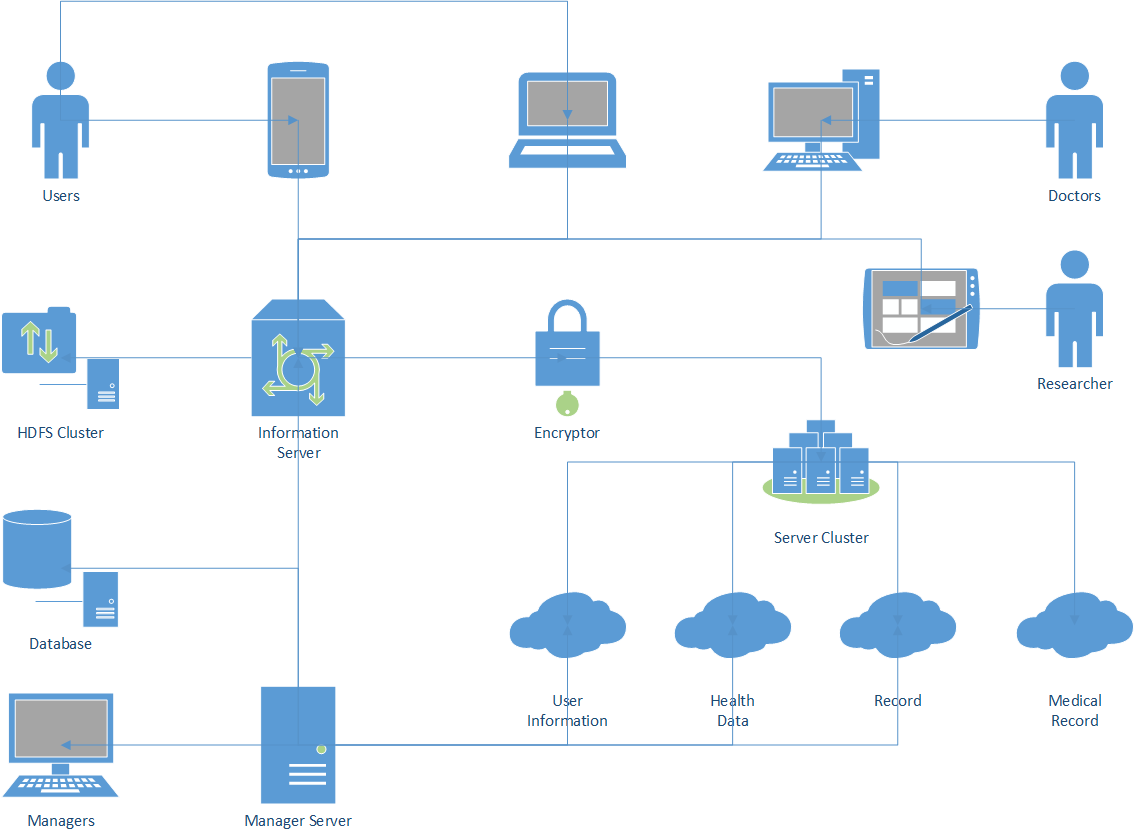
\includegraphics[width=14cm]{figures/arch.png}
        \caption{Architecture}
    \end{figure} 
    \par

\end{document}
% \end{CJK}